\documentclass[journal,12pt,twocolumn]{IEEEtran}
\usepackage[none]{hyphenat}
\usepackage{enumitem}
\usepackage{graphicx}
\usepackage{listings}
\usepackage{kvmap}
\usepackage[utf8]{inputenc}
\usepackage{caption}
\usepackage{hyperref}
\usepackage{watermark}
\usepackage{lipsum}
\usepackage{xcolor}
\usepackage{float}
\usepackage{titlesec}
\usepackage{lmodern}

\title{IMPLEMANTION OF JOHNSON COUNTER USING ARM}
\author{Manoj Chavva- FWC22055}

\begin{document}
\maketitle

\tableofcontents
\vspace{0.5cm}
\begin{abstract}
  This Manual shows the design and Implemantation of four bit Johnson counter by vaman board.
\end{abstract}    
\section{Components}     
\begin{tabular}{|c|c|c|}
    \hline 
      \textbf{S.No} & \textbf{Component} & \textbf{Number}\\
      \hline
	1. & Vaman board & 1 \\
	2. & Bread Board & 1 \\
	3. & Jumper Wires(M-M) & 6 \\
	4. & LED & 4 \\
	5. & USB cable & 1 \\
	
      \hline
      
   \end{tabular}
     \vspace{0.35cm}


\section{Introduction}
\begin{enumerate}
  \item Johnson counters are used to store or process or count the number of events occurred within the circuit.
  \item It is designed with a group of flip-flops, where the inverted output from the last flip-flop is connected to the input of the first flip-flop.
  \item In Johnson counter
  \\No. of states = No. of flip-flop used  
\\Number of used states=2n  
\\Number of unused states=2n - 2*n  
\item Here, the functionality of D flip flop is used for the program. 
\end{enumerate}

    \vspace{2.5cm}   



\section{Circuit Diagram}
\begin{enumerate}
\item The inverted output of the last flip-flop ‘$\bar{Q}$n’ is fed back to the first flip-flop in the sequence bit pattern. 
\item The counter registers cycles in a closed-loop i.e circulates within the circuit.
\begin{figure}[h]
    \centering
    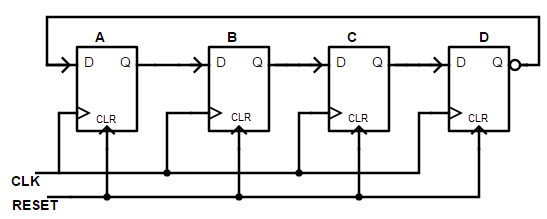
\includegraphics[width=8cm, height=4.2cm]{counter.jpg}
    
    \caption{Four bit Johnson Counter}

\end{figure}
\item Reset pin acts as an on/off switch. So, the flip-flops can be enabled by clicking the Reset switch.

\item CLK pin is used to observe the changes in the output of the flip-flops.
\end{enumerate}



\section{Procedure}
\begin{enumerate}
\item Connect the 4 LED's and vaman according to table \ref{table:1}
\item Observe the states of LED and verify the truth table using the code from the link.



\end{enumerate}


\begin{table}[h]
\centering
\large
\begin{tabular}{|l|l|l|l|l|l|}
\hline
\textbf{vaman} & D2   & D3   & D4   & D5   & GND \\ \hline
\textbf{LED's}   & LED1 & LED2 & LED3 & LED4 &     \\ \hline
\end{tabular}
\caption{Connection Table}
\label{table:1}
\end{table} 





\noindent URL -- \url{https://github.com/ManojChavva/FWC/blob/main/avr-gcc/codes/main.c} 


% Define block styles
\tikzstyle{decision} = [diamond, draw, fill=blue!20, 
    text width=4.5em, text badly centered, node distance=3cm, inner sep=0pt]
%\tikzstyle{block} = [rectangle, draw, fill=blue!20, 
%    text width=5em, text centered, rounded corners, minimum height=4em]
\tikzstyle{block} = [rectangle, draw, 
    text width=5em, text centered, rounded corners, minimum height=4em]

\tikzstyle{line} = [draw, -latex']
\tikzstyle{cloud} = [draw, ellipse,fill=red!20, node distance=3cm,
    minimum height=2em]
    
\begin{tikzpicture}[node distance = 3cm, auto]
    % Place nodes
    \node [block] (init) {vaman};

    \node [block, below of=init, node distance = 4cm] (identify) { LED's};
    
	\node at (4,-2)[block] (delay) {Delay};
\begin{scope}[->,>=latex]
    \foreach \i in {-3,-1,1,3}
    { 

      \draw[->] ([xshift=\i * 0.2 cm]delay.north) |- ([yshift=\i * 0.2 cm]init.east) ;
      \draw[->] ([xshift=\i * 0.2 cm]init.south) -- ([xshift=\i * 0.2 cm]identify.north) ;
       \draw node at (\i * 0.2,-2+\i * 0.2) { \textbullet} ;
       \draw[->] (\i * 0.2,-2+\i * 0.2) -- ([yshift=\i * 0.2 cm]delay.west) ;
      
    }


\foreach [count=\i] \j in {Q1,Q2,Q3,Q4}{
            \node (\i) at ( 0.5-\i * 0.4, -1.0-\i*0.3) {\j} ;
            }

\foreach [count=\i] \j in {D1,D2,D3,D4}{
            \node (\i) at ( 1.6, 1.2-\i*0.4) {\j} ;
            }
    
\end{scope}

 
\end{tikzpicture}

\centering Fig: 2 Sequential Circuit




\section{Truth Table}



\begin{center}
\small   
%    \setlength{\arrayrulewidth}{0.5mm}
%\setlength{\tabcolsep}{18pt}
%\renewcommand{\arraystretch}{1}
\begin{tabular}{|l|l|l|l|l|l|l|l|l|}
\hline
\textbf{CLK} & \textbf{D1} & \textbf{D2} & \textbf{D3} & \textbf{D4} & \textbf{Q1} & \textbf{Q2} & \textbf{Q3} & \textbf{Q4} \\ \hline
0            & 0           & 0           & 0           & 0           & 0           & 0           & 0           & 0           \\ \hline
1            & 1           & 0           & 0           & 0           & 1           & 0           & 0           & 0           \\ \hline
2            & 1           & 1           & 0           & 0           & 1           & 1           & 0           & 0           \\ \hline
3            & 1           & 1           & 1           & 0           & 1           & 1           & 1           & 0           \\ \hline
4            & 1           & 1           & 1           & 1           & 1           & 1           & 1           & 1           \\ \hline
5            & 0           & 1           & 1           & 1           & 0           & 1           & 1           & 1           \\ \hline
6            & 0           & 0           & 1           & 1           & 0           & 0           & 1           & 1           \\ \hline
7            & 0           & 0           & 0           & 1           & 0           & 0           & 0           & 1           \\ \hline
\end{tabular}
   
   \vspace{0.5cm}
   \centering Table II: Truth Table.
\label{table:2}
 \end{center}
 \begin{itemize}
 \item The above table state that
 \end{itemize}
 \begin{enumerate}
 
\item The counter produces the output 0000 when there is no clock input passed(0).
\item  The counter produces the output 1000 when the 1st clock pulse is passed to the flip flops.
 \item  The counter produces the output 1100 when the 2nd clock pulse is passed to the flip flops. \item The counter produces the output 1110 when the 3rd clock pulse is passed to the flip flops.
\item The counter produces the output 1111 when the 4th clock pulse is  passed to the flip flops.
\item  The counter produces the output 0111 when the 5th clock pulse is passed to the flip flops.
\item The counter produces the output 0011 when the 6th clock pulse is passed to the flip flops.
\item The counter produces the output 0001 when the 7th clock pulse is passed to the flip flops.
 \end{enumerate}
 
 
 
\section{Setup}
\begin{enumerate}
\item Connect the Vaman to the Laptop through USB.
\item There is a button and an LED to the left of the USB port on the Vaman.There is another button to the right of the LED.
\item Press the right button first and immediately press the left button.The LED will be blinking green.The Vaman is now in bootloader mode.
\end{enumerate}
\section*{steps for implementation:} 
\begin{enumerate}
\item Login to termux-ubuntu on the android device and execute the following commands:\\
Make sure that the required installation of pygmy-sdk had done prior executing below commands
\begin{lstlisting}
proot-distro login debian
cd  /data/data/com.termux/files/home/
mkdir arm
cd codes/GCC_Project
make
scp /data/data/com.termux/files/home/
arm/codes/GCC_Project/output/bin/codes.bin 
usernameofpc@IPaddress:/home/username
\end{lstlisting}
%svn co https://github.com/velicharlagokulkumar/FWC_module1/trunk/arm/codes

Make sure that the appropriate username,IP address of the Laptop is given in the above command.
\item Now execute the following commands on the Laptop terminal\\
Make sure that required installation of programmer application and modification of bash file had done prior executing below command
\begin{lstlisting}
bash flash.sh codes.bin
\end{lstlisting}
\item After finishing the process of flashing with the programmer application press the button to the right of the USB port to reset. Vaman is now flashed with our source code
\end{enumerate}
\end{document} 
 
 
 \section*{Conclusion}
 Thus the Johnson counter designed and Implemented.

\end{document}
